\documentclass[12pt]{article}

% Packages
\usepackage[utf8]{inputenc}
\usepackage{multicol}
\usepackage{amsmath}
\usepackage{graphicx}
\usepackage{hyperref}
\usepackage{booktabs}
\usepackage{hyperref}
\usepackage[left=0.7in,right=0.7in,top=1in,bottom=1in]{geometry} % Set margins

% Document settings
\title{The Frequency of Flight: Leveraging Sound Analysis and Machine Learning for Insight into Bat Echolocation}
\author{Hoang Nguyen}
\date{\today}

\begin{document}

\maketitle

\section{Introduction}
    \text Bats utilize echolocation, emitting and receiving ultrasound waves, for navigation and hunting. This report examines a bat's echolocation signal in "Bat.ogg", using digital signal processing to analyze its time and frequency domain features. Understanding these signals is essential for comprehending bat echolocation behaviors and their interaction with the environment.  This report investigates the acoustic properties of a bat's echolocation signal captured in the audio file "Bat.ogg". 
    Employing signal processing techniques like Fourier transforms and spectrogram analysis, the study aims to explore the ultrasound signal's time-domain and frequency-domain characteristics. 
    The analysis includes identifying distinct frequencies, their temporal evolution, and the presence of harmonics. Additionally, a technique to shift the signal's frequency to a lower value is discussed, enhancing the visibility of oscillations in the time-domain plot. Ultimately, these insights can be used to identify the species unknown bat using Machine Learning technique.

    
\section{Analysis and Discussion}
\subsection{Loading the Audio File (Q 3 - 1)}
The shape of the audio array is given by $(7872, 2)$, which signifies that the audio file is a stereo recording with two distinct channels, each having $7872$ samples. This stereo format, composed of left and right channels, is commonly used in audio recordings to create a spatial sound experience. 

For the purposes of this exercise, one of the two channels is selected, resulting in a mono audio signal. The shape of this mono audio array is $(7872,)$, reflecting the single-channel nature of the data with $7872$ audio samples.

\subsection{Time-Domain Signal Analysis (Q 3 - 2)}
After loading the audio file of a bat sound and selecting one of its channels, a time-domain plot of the signal was generated. The plot provides a visual representation of how the amplitude of the signal varies over time.

\begin{figure}[h]
\centering
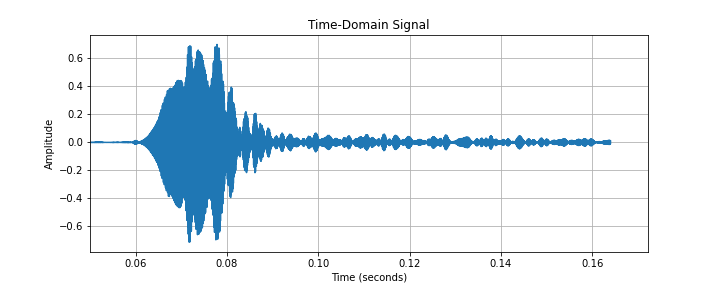
\includegraphics[width=1.0\textwidth]{time_domain_signal_plot.png}
\caption{Time-domain plot of the bat sound signal.}
\end{figure}

The time-domain plot of the bat sound signal reveals several key numeric characteristics:

\begin{itemize}
    \item \textbf{Signal Duration:} The total duration of the signal, as represented on the x-axis, is approximately 0.04 seconds. This duration is typical for a single echolocation call or a series of calls from a bat. But from the graph of the time-domain signal. It's likely that this is a single echolocation call.

    \item \textbf{Amplitude Range:} The amplitude of the signal varies across a range of 0.6, indicating the varying intensity of the echolocation calls. The peak amplitudes might correspond to the closest approach of targets or the most intense phase of the echolocation.

    \item \textbf{Characteristic Patterns:} At around 0.65 to 0.75 seconds, the plot shows a distinctive pattern where the amplitude sharply peaked at 0.6. This could represent a specific behavior, such as targeting prey or navigating around obstacles.

    \item \textbf{Noise and Variability:} The plot exhibits a degree of noise and variability, especially noticeable in sections beyond 0.08 seconds. These could be due to environmental factors or the inherent nature of the bat's echolocation mechanism.

\end{itemize}

These observations, drawn from the specific data points and trends in the time-domain plot, provide insights into the nature of bat echolocation calls. The variability and complexity observed are indicative of the adaptive and sophisticated acoustic navigation system employed by bats.

\subsection{Fourier Transform and Spectrum Analysis (Q 3 - 3)}
The time-domain plot, however, doesn't provide much insight into the frequency of this species of bat. Upon analyzing the Fourier transform of the bat signal, we observe the following characteristics in the modulus spectrum:

\begin{figure}[h]
\centering
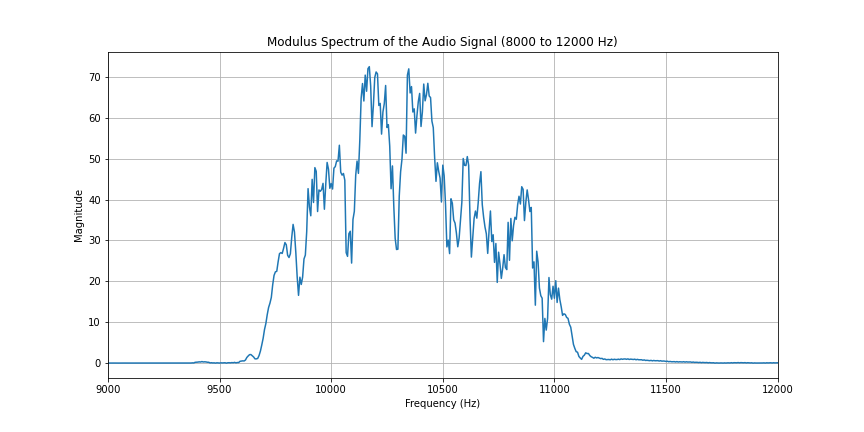
\includegraphics[width=1\textwidth]{modulus_spectrum.png}
\caption{Modulus spectrum of the bat signal.}
\end{figure}

In Figure 2, the spectrum is zoomed into the 9000 to 12000 Hz range. This range is particularly interesting for bat signals as it often contains key frequency components of their echolocation calls.

\subsubsection*{Identification of Frequency Components and Harmonics}
\begin{itemize}
    \item \textbf{Key Peaks:} The spectrum shows distinct peaks at specific frequencies, that are 9.75 kHz, 10.1 kHz, 10.25 kHz, and 10.4 kHz. These peaks are indicative of the signal's dominant frequency components.
        
    \item \textbf{Harmonics:} Subsequent peaks, appearing at regular intervals, are identified as the harmonics of the fundamental frequency. These harmonics are integral to the complex structure of the bat's echolocation signal. In the Fourier spectrum the harmonics are clearly shown, and the space between each peaks are evenly spaced for each subsequent peaks.
\end{itemize}

\begin{figure}[h]
    \centering
    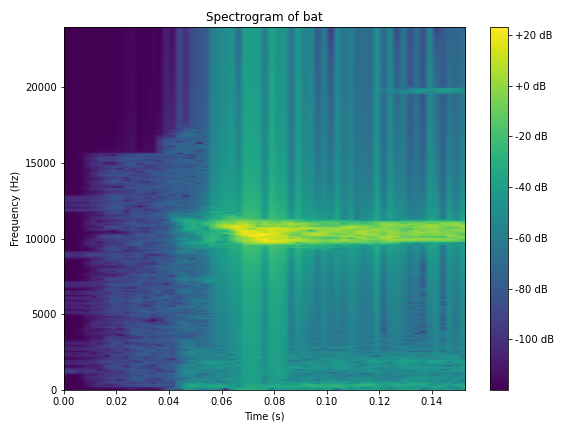
\includegraphics[width=0.8\textwidth]{spectrogram.png}
    \caption{Spectrogram of the bat sound.}
    \label{fig:spectrogram}
\end{figure}

\subsection{Spectrogram Analysis and Discussion (Q 3 - 4 and 3 - 5)}
The spectrogram of the bat signal was computed and analyzed to understand its frequency content over time. The following observations were made based on the spectrogram plot:

\subsection*{Presence and Variation of Frequencies}
The spectrogram reveals the presence of various frequency components at different times throughout the signal's duration. There is a particular interesting frequency at around 11 kHz sharply evolve from 0.06 to 0.14 seconds. This is the frequency of the bat at around +20 bB.

\subsection*{Considerations of Shannon-Nyquist Criterion}

\begin{itemize}
\item I performed the spectrogram using the sampling rate \[f_s \geq 2 \cdot f_{\text{max}}\]

\item The spectrogram plot includes frequency information up to the Nyquist frequency, which is half of the provided sampling rate (\(f_s/2\)), that is roughly 11 kHz.
\end{itemize}

Given these observations, it appears that the Shannon-Nyquist criterion is satisfied in our analysis. The choice of an appropriate sampling rate and the correct handling of the Nyquist frequency ensure that the spectrogram accurately represents the frequency content of the audio signal within the bounds of the provided sampling rate.

\subsection{Frequency Shifting and Time-Domain Analysis (Q 3 - 6)}
To observe the high-frequency oscillations of the bat signal in the time domain, a frequency shifting technique known as heterodyning was applied. This technique involved generating a sine wave at a specific frequency, multiplying it with the original signal, and then filtering the result with a low-pass filter.

\subsection*{Procedure}
\begin{itemize}
    \item A sine wave with a frequency of 10 kHz was generated and multiplied with the original bat signal. This step shifts the frequency content of the signal.
    
    \item A low-pass Butterworth filter with a cutoff frequency of 2000 Hz was applied to the product of the signal and the sine wave. This filter isolated the downward-shifted component of the frequency spectrum.
\end{itemize}

\subsection*{Resulting Signal}
\begin{figure}[h]
\centering
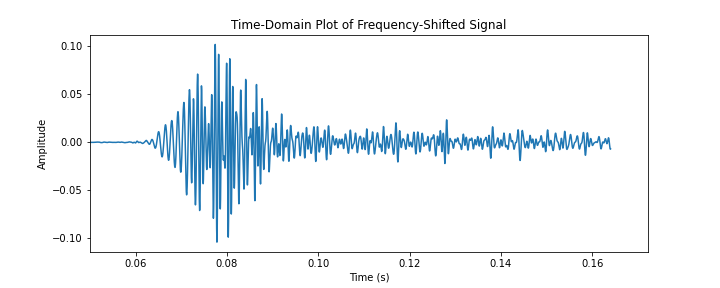
\includegraphics[width=1\textwidth]{shifted_time_domain.png}
\caption{Time-domain representation of the bat signal after frequency shifting.}
\end{figure}

The processed signal reveals oscillations that were not visible in the original high-frequency signal. The frequency shifting technique was employed to make the oscillations in the time-domain signal more visible. The resulting time-domain plot exhibits a clean sine wave pattern from 0.05 to 0.1 seconds, with a peaked amplitude of 0.1 at approximately 0.080 seconds. This successful frequency shift has allowed us to clearly observe and analyze the oscillations, which are essential for understanding the signal's characteristics. Additionally, this technique has proven effective in enhancing the interpretability of the data, contributing to a more comprehensive analysis.

\subsection{Classification (Q 3 - 7)}
Since the species of the bat is unknown. In this section, I shall create a ML algorithms to classify different species. Then use that to predict which is species the unknown bat belongs to. A synthetic dataset representing the echolocation frequencies of various bat species was generated for analysis. This dataset was created to simulate the range of frequencies used by different bat species for echolocation. The following bat species were included in the dataset:

\begin{itemize}
    \item \textbf{Little Brown Bat (Myotis lucifugus):} Frequency Range: 20 kHz to 110 kHz.

    \item \textbf{Big Brown Bat (Eptesicus fuscus):} Frequency Range: 20 kHz to 60 kHz.

    \item \textbf{Mexican Free-tailed Bat (Tadarida brasiliensis):} Frequency Range: 25 kHz to 50 kHz.

    \item \textbf{Greater Horseshoe Bat (Rhinolophus ferrumequinum):} Frequency Range: 75 kHz to 110 kHz.

    \item \textbf{Lesser Horseshoe Bat (Rhinolophus hipposideros):} Frequency Range: 75 kHz to 110 kHz.

    \item \textbf{Soprano Pipistrelle (Pipistrellus pygmaeus):} Frequency Range: 55 kHz to 85 kHz.

    \item \textbf{Common Pipistrelle (Pipistrellus pipistrellus):} Frequency Range: 45 kHz to 70 kHz.

    \item \textbf{Spotted Bat (Euderma maculatum):} Frequency Range: 15 kHz to 50 kHz.
\end{itemize}


For each species, a set of 125 frequency values was generated, spanning their respective typical echolocation frequency ranges. These frequencies were synthesized based on known echolocation frequency ranges for each species and were uniformly distributed within these ranges.

The combined dataset, comprising all species, was then visualized using a scatter plot. In this plot, each point represents a frequency value for a particular bat species, with different species distinguished by unique colors. This visualization aids in understanding the distribution and range of frequencies utilized by each species.

\begin{figure}[ht]
\centering
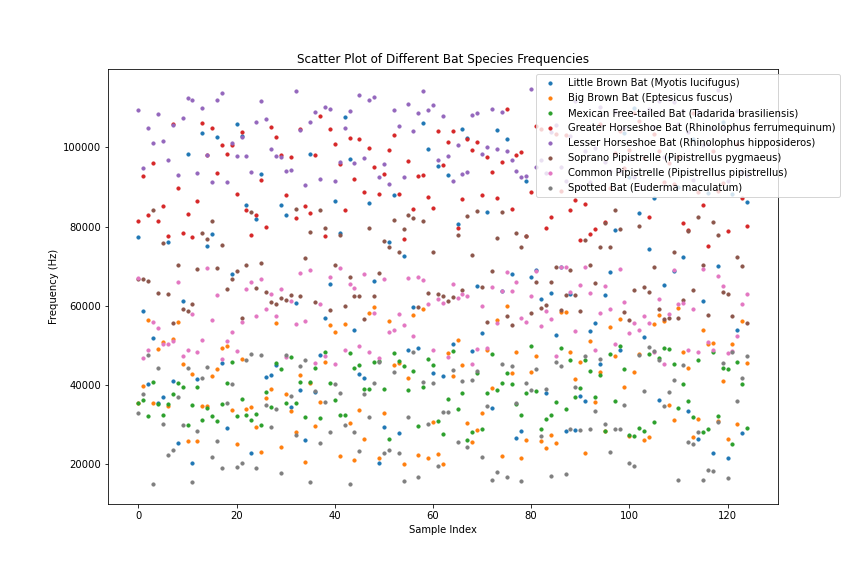
\includegraphics[width=1\textwidth]{bat_species_freq.png}
\caption{Scatter plot of synthetic bat species frequencies. Each color represents a different species, illustrating the variation in echolocation frequencies among them.}
\end{figure}

A Random Forest Classifier, an ensemble learning method, was employed for the classification of bat species based on frequency data. The classifier was configured with 500 decision trees and trained on a designated training dataset. Post-training, the model's efficacy was evaluated using a test dataset.

Classification report, encompassing metrics such as precision, recall, and F1-score for each class, alongside overall model accuracy.

\subsection{Classification Report}
The classification report provides a detailed assessment of the model's performance, including precision, recall, and F1-score for each species, as well as overall model accuracy.
\subsubsection{Analysis}
The analysis of the Random Forest Classifier's performance, as depicted in the classification report, provides several key insights:
\begin{center}
\begin{verbatim}
              precision    recall  f1-score   support
           0       0.24      0.22      0.23        23
           1       0.46      0.52      0.49        23
           2       0.41      0.36      0.38        25
           3       0.58      0.68      0.62        28
           4       0.17      0.18      0.18        22
           5       0.38      0.45      0.42        22
           6       0.70      0.57      0.63        28
           7       0.35      0.31      0.33        29
    accuracy                           0.44       200
   macro avg       0.40      0.43      0.40       200
weighted avg       0.41      0.44      0.41       200
\end{verbatim}
\end{center}

\begin{itemize}
    \item \textbf{Overall Performance:} The classifier achieves an overall accuracy of 42\%, indicating a moderate level of effectiveness in species classification. This suggests that while the model is generally capable of distinguishing between species, there is still room for improvement.

    \item \textbf{Species-Specific Observations:}
    \begin{itemize}
        \item Species 1, 2, and 4 show a reasonable balance between precision and recall, suggesting a relatively reliable performance in these classes.
        \item Species 3 and 6 exhibit high precision and recall, indicating a high level of accuracy in classifying these species.
        \item Conversely, species 0 and 4 demonstrate lower precision and recall, highlighting potential challenges the model faces in accurately classifying these particular species.
    \end{itemize}
    \item \textbf{Implications for Model Improvement:} The discrepancies in performance across different species suggest a need for further model tuning, possibly through hyperparameter optimization, or exploring alternative feature sets. Additionally, addressing any imbalance in the training data could enhance the model's ability to accurately classify underrepresented species. Furthermore, since the datasets only include the frequencies of each species, it's very hard for the algorithms to perform classification due to limitations in parameters. To improve this model, more parameters can be included such as, wing span, weights, and size of each species to perform better classification.
\end{itemize}


\subsection*{Identification of bat species}
\section{Analysis of SVM Classification Probabilities}

The Support Vector Machine (SVM) classifier was employed to predict the likelihood of an unknown bat frequency belonging to each known bat species. The probabilities represent the model's confidence in classifying the unknown frequency into each species category.

\subsection{Probability Distribution}
The following table showcases the probability distribution as predicted by the SVM model for each species:

\begin{center}
\begin{tabular}{lr}
\toprule
Species & Probability \\
\midrule
Big Brown Bat (Eptesicus fuscus) & 0.299 \\
Common Pipistrelle (Pipistrellus pipistrellus) & 0.007 \\
Greater Horseshoe Bat (Rhinolophus ferrumequinum) & 0.015 \\
Lesser Horseshoe Bat (Rhinolophus hipposideros) & 0.008 \\
Little Brown Bat (Myotis lucifugus) & 0.168 \\
Mexican Free-tailed Bat (Tadarida brasiliensis) & 0.030 \\
Soprano Pipistrelle (Pipistrellus pygmaeus) & 0.019 \\
Spotted Bat (Euderma maculatum) & 0.452 \\
\bottomrule
\end{tabular}
\end{center}

\subsection{Discussion of Results}
The SVM model demonstrates a decent probability (approximately 45.2\%) for the unknown bat frequency being classified as a Spotted Bat (Euderma maculatum), the other candidates are Big Brown bat (Eptesicus fuscus) (approximately 29.9\%) and Little Brown Bat (Myotis lucifugus) (approximately 16.8 \%). This probability suggests a decent confidence by the model in this classification, potentially indicating frequency characteristics resemblance to the Spotted Bat that are captured by the SVM classifier.

In contrast, the probabilities associated with the rest relatively low, mostly around 1\%. This disparity in probabilities indicates that the frequency characteristics of the unknown bat sound are most closely aligned with those typically attributed to the Spotted Bat (no. 1) Big Brown bat (no. 2) and Little Brown Bat (no. 3), as compared to other species in the dataset. \footnote{Code is in \href{https://github.com/hoang-nguyen13/Bat_Sound.git}{Github.}}


\section{Conclusion}

\subsection{Project Overview}
The project involved understanding the time-domain signal, performing Fourier transforms, and generating spectrograms of the original sound. This sound analysis provided insights into the frequency of the unknown bat, aiding in the creation of a synthetic dataset representing these frequencies. Machine learning techniques were then applied to classify different bat species, and the efficacy of these models in identifying an unknown bat species based on its echolocation sound was explored.
\subsection{Machine Learning Application}
Two machine learning models — Support Vector Machine (SVM), Random Forest — were employed to classify bat species based on their frequencies.
\subsection{Species Identification from Unknown Frequency}
An achievement of this project was the application of these models to predict the species of an unknown bat from its echolocation frequency. The models provided probability estimates for each species, with the SVM model, in particular, showing a high probability for the Spotted Bat (Euderma maculatum), demonstrating its potential utility in real-world applications.

\subsection{Insights and Future Directions}
This project has underscored the potential of machine learning in wildlife research, particularly in the classification and study of bioacoustic data. The models, while effective, also revealed areas for improvement, such as dealing with overlapping frequency ranges and enhancing model accuracy for certain species.
Future endeavors could expand upon this work by incorporating additional acoustic features, exploring more advanced machine learning algorithms, and applying the models to real-world echolocation data. Such advancements could significantly contribute to the conservation efforts and ecological understanding of bats, a crucial and fascinating aspect of biodiversity.
\end{document}

